% copyright 2020 Edmundo Carmona Antoranz
% Released under the terms of Creative Commons Attribution-ShareAlike 4.0 International Public License

\section{La intención es lo que cuenta}
\label{intent}
Ya no hay necesidad de mostrar el ancestro y las ramas por separado. Solo mostrar el archivo con conflicto
o el {\bf CB} debería ser suficiente. Tomemos este ejemplo de un conflicto:

\subsection{Ejemplo 4 - conflicto sobre nuestro adorado script}
\label{example_04}

\begin{lstlisting}[style=python_style, caption={\bf Ejemplo 4}]
#!/usr/bin/python

import sys

colors = {"black": "black mirror",
          "white": "white noise",
          "blue": "blue sky"}

def getPhrase(color):
<<<<<<< HEAD
    phrase = "%s: %s" % (color, colors[color])
    return phrase
||||||| c8bf13a
    phrase = colors[color]
    return phrase
=======
    if color in colors:
        phrase = colors[color].upper()
        return phrase
    else:
        sys.stderr.write("%s is not a known color\n" % color)
        sys.exit(1)
>>>>>>> example4/branchB

print(getPhrase(sys.argv[1]))
\end{lstlisting}

Se podría resolver como lo hemos hecho hasta ahora. Se comienza a trabajar en el {\bf UB}\footnote{Se incluyen
los marcadores de conflicto para dar claridad}:
\begin{lstlisting}[style=python_style, firstnumber=10, caption={\bf Ejemplo 4} - Paso 1 - UB]
<<<<<<< HEAD
    phrase = "%s: %s" % (color, colors[color])
    return phrase
||||||| c8bf13a
\end{lstlisting}

Ahora consideramos el {\bf dML}:
\begin{lstlisting}[style=python_style, firstnumber=13, caption={\bf Ejemplo 4} - Paso 2 - dML]
||||||| c8bf13a
    phrase = colors[color]
    return phrase
=======
    if color in colors:
        phrase = colors[color].upper()
        return phrase
    else:
        sys.stderr.write("%s is not a known color\n" % color)
        sys.exit(1)
>>>>>>> example4/branchB
\end{lstlisting}
{\bf dML}: Hay una nueva condición que verifica que el color esté definido (línea 17). Si no existe, cae en el bloque {\it else}
(líneas 20-22). Las líneas preexistentes se colocaron dentro del condicional y se ajustó su indentación por esa razón (líneas
18-19). Primero, copiemos esas líneas desde el {\bf LB} hacia el {\bf UB}.

\begin{lstlisting}[style=python_style, firstnumber=10, caption={\bf Ejemplo 4} - Paso 3 - Copiar desde el LB]
<<<<<<< HEAD
    if color in colors:
        phrase = colors[color].upper()
        return phrase
    else:
        sys.stderr.write("%s is not a known color\n" % color)
        sys.exit(1)
||||||| c8bf13a
\end{lstlisting}
{\bf Casi} lo tenemos. Pero hay un problema: Como copiamos el contenido {\it verbatim}, perdimos la línea del {\bf UB}
donde se estaba cambiando la frase para incluir el color original. Miren el {\bf UB} antes de comenzar a resolver de nuevo (línea 11):

\begin{lstlisting}[style=python_style, firstnumber=10, caption={\bf Ejemplo 4} - Paso 1 - UB]
<<<<<<< HEAD
    phrase = "%s: %s" % (color, colors[color])
    return phrase
||||||| c8bf13a
\end{lstlisting}

Ok, entonces debemos poder reemplazar la línea donde colocamos el valor desde el diccionario y con eso estaría bien:
\footnote{Eso es, {\bf si} hubieran sido suficientemente cuidadosos de guardar el contenido del {\bf UB}. Como probablemente no lo hicieron,
tocaría comenzar a resolver el conflicto desde el principio}
\begin{lstlisting}[style=python_style, firstnumber=10, caption={\bf Ejemplo 4} - Paso 4 - Editar el UB]
<<<<<<< HEAD
    if color in colors:
        phrase = "%s: %s" % (color, colors[color])
        return phrase
    else:
        sys.stderr.write("%s is not a known color\n" % color)
        sys.exit(1)
||||||| c8bf13a
\end{lstlisting}

Eso {\bf tampoco} es correcto. Ahora se pierde la llamada a {\bf upper()} que viene del {\bf LB}. Así que no podemos copiar cambios
{\bf verbatim} de un bloque al otro? Todo depende de lo que se traten los cambios. En este caso la línea está recibiendo
cambios por las dos ramas así que debemos considerar la {\bf intención} de ambas, no los cambios literales.

Comencemos a resolver el conflicto desde el principio, en el {\bf UB}:
\begin{lstlisting}[style=python_style, firstnumber=10, caption={\bf Ejemplo 4} - Paso 1 - UB]
<<<<<<< HEAD
    phrase = "%s: %s" % (color, colors[color])
    return phrase
||||||| c8bf13a
\end{lstlisting}

El {\bf dML} (paso 2) no ha cambiado. Una nueva condición se agregó y la copiamos en el paso 3:
\begin{lstlisting}[style=python_style, firstnumber=10, caption={\bf Ejemplo 4} - Paso 3 - Conditional]
<<<<<<< HEAD
    if color in colors:
    phrase = "%s: %s" % (color, colors[color])
    return phrase
||||||| c8bf13a
\end{lstlisting}

Necesitamos ajustar la indentación de las lineas como se hizo en {\bf la otra rama}:
\begin{lstlisting}[style=python_style, firstnumber=10, caption={\bf Ejemplo 4} - Paso 4 - Adjustar indentación]
<<<<<<< HEAD
    if color in colors:
        phrase = "%s: %s" % (color, colors[color])
        return phrase
||||||| c8bf13a
\end{lstlisting}

Agregamos la llamada a {\bf upper()}:
\begin{lstlisting}[style=python_style, firstnumber=10, caption={\bf Ejemplo 4} - Paso 5 - llamada a {\bf upper()}]
<<<<<<< HEAD
    if color in colors:
        phrase = "%s: %s" % (color, colors[color].upper())
        return phrase
||||||| c8bf13a
\end{lstlisting}

Agregamos el bloque {\it else}:
\begin{lstlisting}[style=python_style, firstnumber=10, caption={\bf Ejemplo 4} - Paso 6 - bloque {\bf else}]
<<<<<<< HEAD
    if color in colors:
        phrase = "%s: %s" % (color, colors[color].upper())
        return phrase
    else:
        sys.stderr.write("%s is not a known color\n" % color)
        sys.exit(1)
||||||| c8bf13a
\end{lstlisting}
Y ahora llegamos a la solución del conflicto. Remuevan las otras partes del conflicto y los marcadores:

\begin{lstlisting}[style=python_style, caption={\bf Ejemplo 4} - final]
#!/usr/bin/python

import sys

colors = {"black": "black mirror",
          "white": "white noise",
          "blue": "blue sky"}

def getPhrase(color):
    if color in colors:
        phrase = "%s: %s" % (color, colors[color].upper())
        return phrase
    else:
        sys.stderr.write("%s is not a known color\n" % color)
        sys.exit(1)

print(getPhrase(sys.argv[1]))
\end{lstlisting}

Pero entonces, si no podemos copiar código de una rama a la otra, como hacemos el trabajo? El truco es {\bf replicar los cambios}
que fueron incluidos en el {\bf dML} y colocarlos en el {\bf UB}, no copiar los cambios.

Este trabajo donde se debe analizar {\bf cuidadosamente} lo que ha cambiado (palabra por palabra, espacio por espacio, tab a tab,
paréntesis a paréntesis, condicional a condicional) debe ser hecho en cada uno de los conflictos a los que se enfrenten. Me encantaría
darles un truco para pode hacer este trabajo más sencillo... pero no lo hay. Una herramienta valiosa que podrían utilizar
bajo ciertas circunstancias es usar {\bf git diff --color-words} para comparar {\bf el ancestro común} con las ramas... o incluso
las ramas entre ellas:
\footnote{Fíjense como uso las propias ramas como parámetros {\bf y} también en el uso del triple punto {\bf (...)}. Eso es para que
git no compare las ramas entre allas sino {\bf el ancestro común} de ambas ramas contra la segunda rama usada como arfumento. Eso es para
no tener que calcular cual es {\bf el ancestro común} (git provee la revisión de {\bf el ancestro común} en unos conflictos, pero
no en otros, por si acaso).}


% TODO add terminal output instead of the images
\begin{figure}
	\centering
	\caption{Diferencias introducidas por la rama {\bf branchA}}
	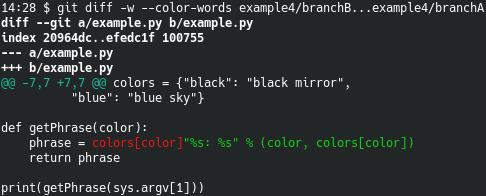
\includegraphics{color_words_02.png}
	\caption{Diferencias introducidas por la rama {\bf branchB}}
	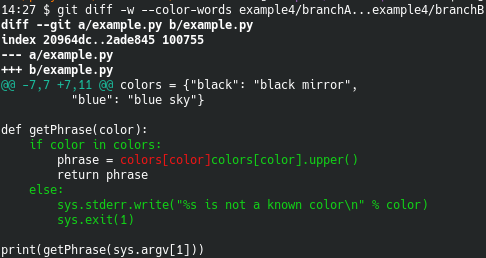
\includegraphics{color_words_01.png}
\end{figure}

Cuando las personas deciden no hacer este trabajo exhaustivamente, fácilmente se escapan detalles de las ramas involucradas
(o se copia cambios {\it verbatim} borrando otros cambios) y eso es lo que eventualmente podría reventar tiempo después, algunas
veces de forma {\it GRANDE.... ESPECTACULAR... FULGURANTE.... {\bf en producción}}. Ciertamente no el mejor sitio para
enterarse de que no se trajo un cambio en un merge hace algunas semanas o meses.

Si se agrega código a una rama, probablemente debería quedar en el código resultante, justo como hicimos con la sección {\bf else}
\footnote{No estoy diciendo copiar verbatim. Podría ser necesario hacer ajustes. El nombre de una variable cambió? Adivinen
lo que tendrán que hacer}. Y el código borrado es un caso especial que debe ser analizado cuidadosamente por lo que estaré
abordándolo más adelante.

\subsection{Ejercicios}
\subsubsection{Ejercicio 4 - un conflicto en git}
Del \hyperref[git_repo]{repo de git}, hagan checkout de la revisión {\bf d9d65e9f6a} y hagan {\it merge} de {\bf b57e8119e6}.
\footnote{Estos son los padres de la revisión {\bf 01f8d78887}} La solución está \hyperref[exercise_04]{aquí}.

\subsubsection{Ejercicio 5 - otro conflicto en git}
Del \hyperref[git_repo]{repo de git}, hagan checkout de la revisión {\bf cf054f817a} y hagan {\it merge} de {\bf caf388caa1}.
\footnote{Estos son los padres de la revisión {\bf 9b6606f43d}} La solution está \hyperref[exercise_05]{aquí}.
